{
% Set colour theme to an ominous white-on-black
\DarkMode
\begin{frame}
    \frametitle{The big picture}
    \framesubtitle{Biology is sometimes compared to physics}

    \begin{center}
        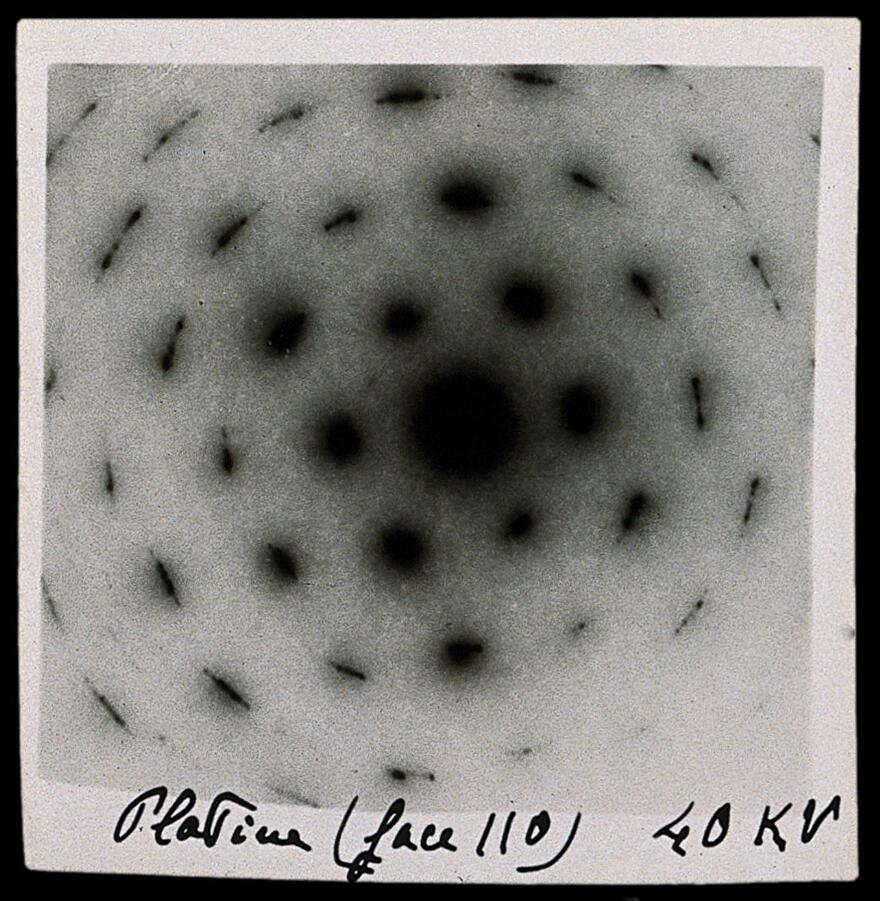
\includegraphics[height=0.80\textheight]{figures/JJTrillat_ElectronDiffractionPt.jpg}
    \end{center}
\footnotetext[1]{https://wellcomecollection.org/works/gc6a9472}
\end{frame}
}

{
\DarkMode
\begin{frame}
    \frametitle{The big picture}
    \framesubtitle{But physics is about 400 years old}

    \begin{columns}
        \begin{column}{0.5\textwidth}
        \begin{center}
            \tiny{Equations of motion}
        \end{center}
        \end{column}
        \begin{column}{0.5\textwidth}
        \begin{center}
            \tiny{Inv. square laws}
        \end{center}
        \end{column}
    \end{columns}

    \begin{columns}
        \begin{column}{0.5\textwidth}
            % planets orbiting
        \end{column}
        \begin{column}{0.5\textwidth}
            % cavendish torsion balance
        \end{column}
    \end{columns}

\begin{center}
    Fundamentals: \textbf{1600s}
\end{center}
\end{frame}
}

{
\DarkMode
\begin{frame}
    \frametitle{The big picture}
    \framesubtitle{And biology/medicine is about 200 years old}

    \begin{columns}
        \begin{column}{0.5\textwidth}
            \begin{center}
                \small{Genetics}
            \end{center}
        \end{column}
        \begin{column}{0.5\textwidth}
            \begin{center}
                \small{Cell theory}
            \end{center}
        \end{column}
    \end{columns}

    \begin{columns}
        \begin{column}{0.43\textwidth}
        % some varieties of pea
            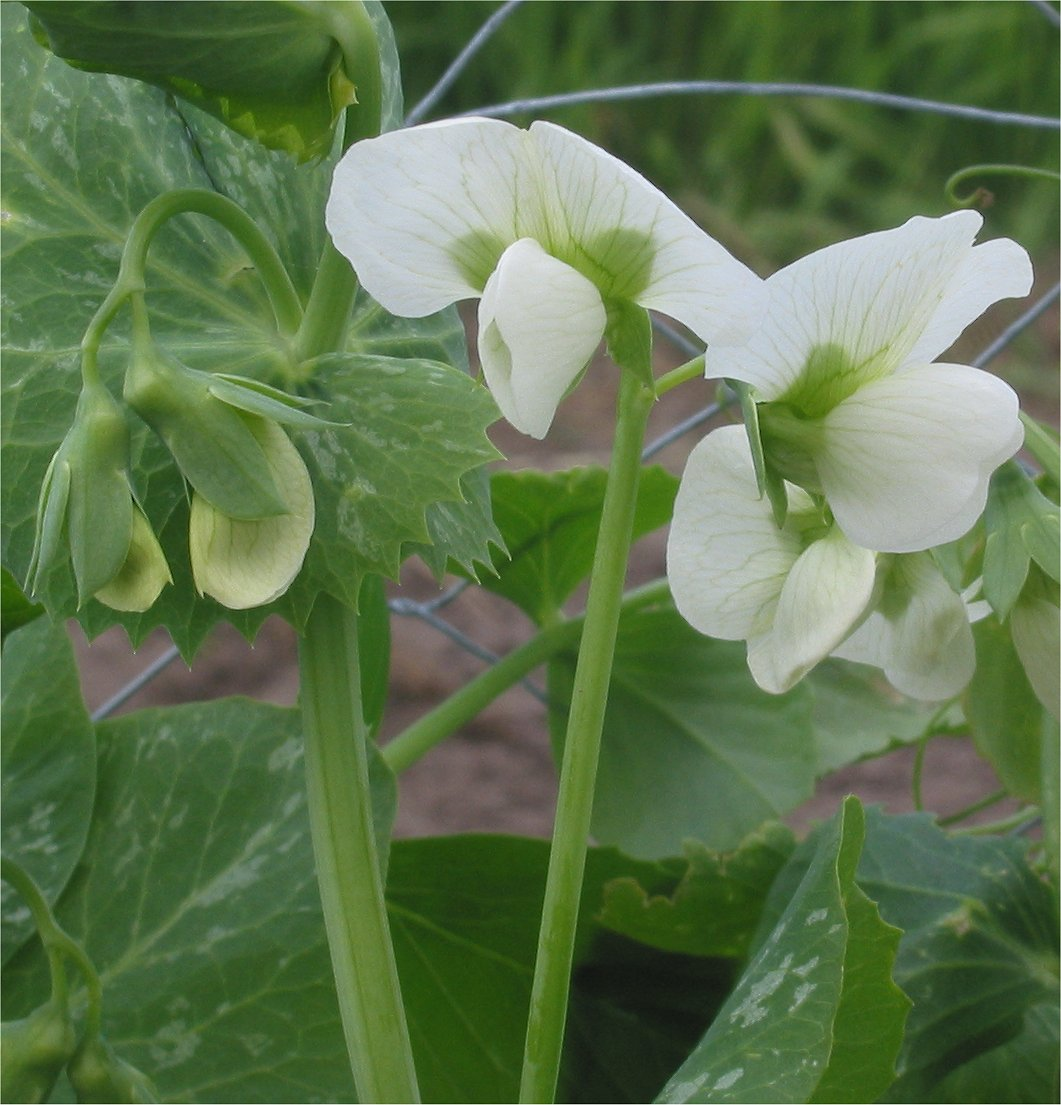
\includegraphics[width=\textwidth]{figures/Doperwt_rijserwt_bloemen_Pisum_sativum.jpg}
        \end{column}
        \begin{column}{0.57\textwidth}
            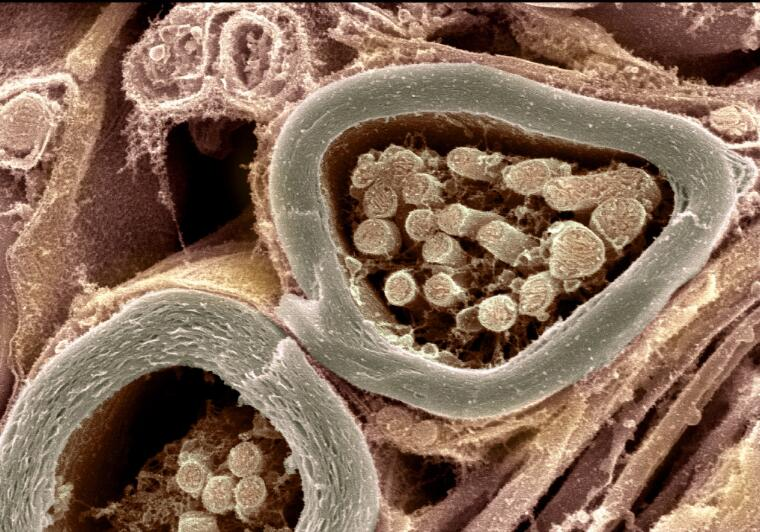
\includegraphics[width=\textwidth]{figures/myelin.jpg}
        \end{column}
    \end{columns}

\begin{center}
    Fundamentals: \textbf{1800s}
\end{center}

\footnotetext[1]{https://commons.wikimedia.org/wiki/User:Rasbak}
\footnotetext[2]{https://wellcomecollection.org/works/ugyj9njv}
\end{frame}
}

{
\DarkMode
\begin{frame}
    \setbeamercolor{item}{fg=white}
    \setbeamercolor{normal text}{fg=white}
    \usebeamercolor[fg]{normal text}
    \frametitle{The big picture}
    \framesubtitle{The value of mechanistic models}
    \begin{columns}
        \begin{column}{0.5\textwidth}
        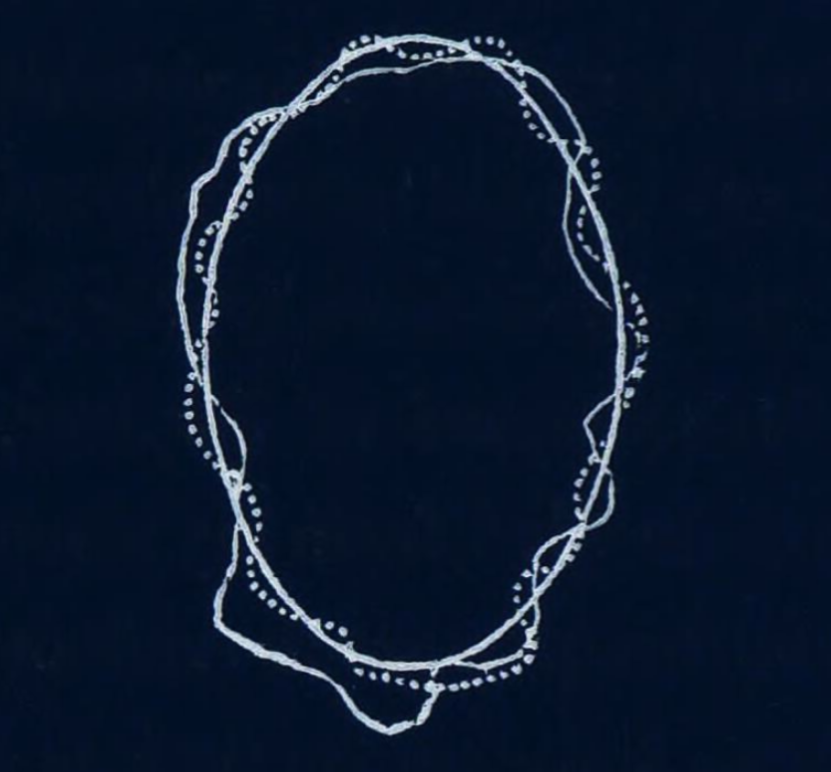
\includegraphics[width=\textwidth]{figures/Orbit2_Wellcome-inv.png}
        %\begin{center}
        %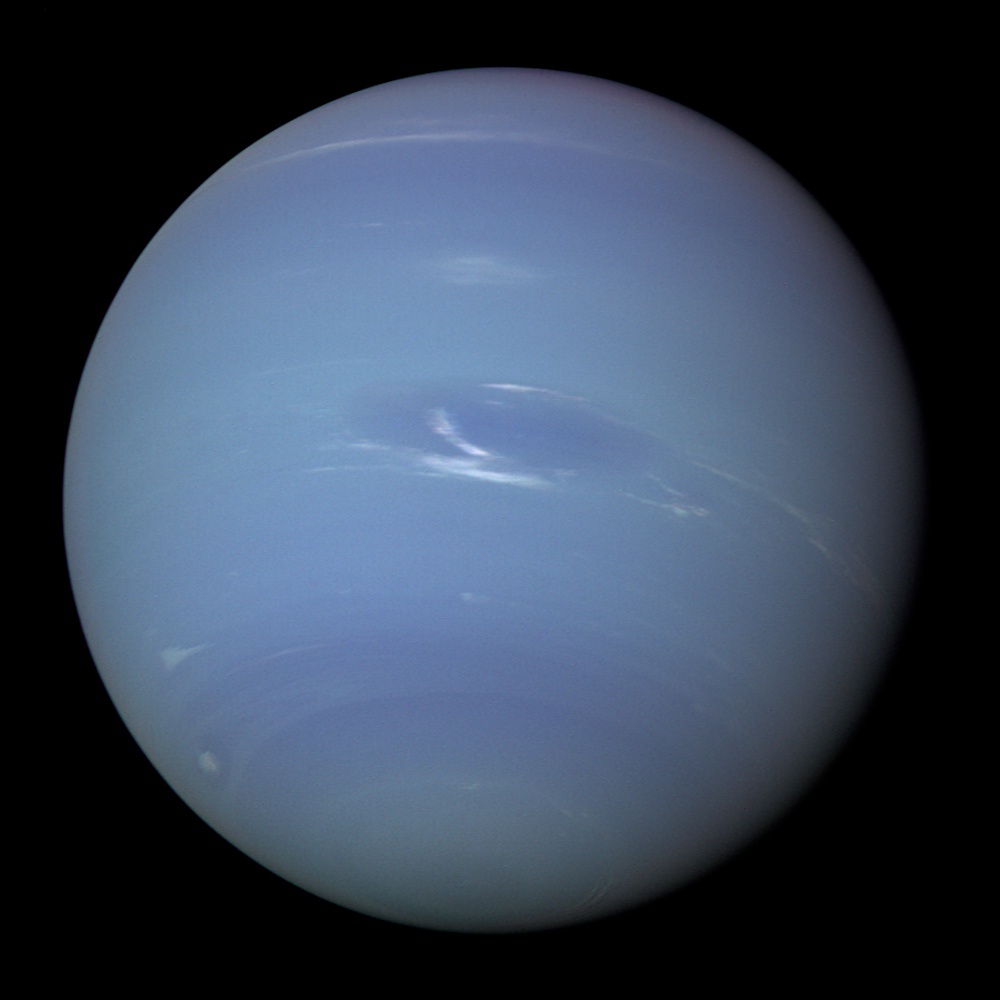
\includegraphics[width=0.65\textwidth]{figures/Neptune_-_Voyager_2_(29347980845)_flatten_crop.jpg} 
        %\end{center}

        %$\uparrow$ within $1^\circ$ of predicted location
        \end{column}
        \begin{column}{0.5\textwidth}
        \begin{itemize}
            \item Model with specific mechanism
            \item Exhausted known factors
            \item Residuals = new factor
            \item Model predicted \emph{size and location} of unknown planet
        \end{itemize}
        \end{column}
    \end{columns}
\footnotetext[1]{J.P. Nichol, ``The planet Neptune: an exposition and history''
1849}
\end{frame}
}

{
\DarkMode
\begin{frame}
    \setbeamercolor{item}{fg=white}
    \setbeamercolor{normal text}{fg=white}
    \usebeamercolor[fg]{normal text}
    \frametitle{The big picture}
    \framesubtitle{The value of mechanistic models}
    \begin{columns}
        \begin{column}{0.5\textwidth}
        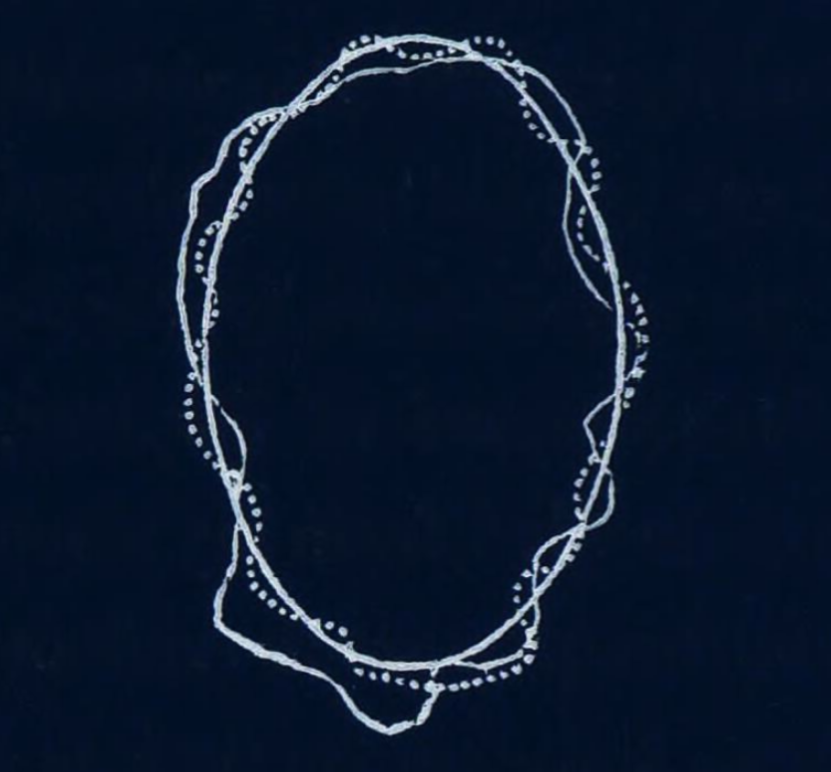
\includegraphics[width=\textwidth]{figures/Orbit2_Wellcome-inv.png}
        \end{column}
        \begin{column}{0.5\textwidth}
        \begin{center}
        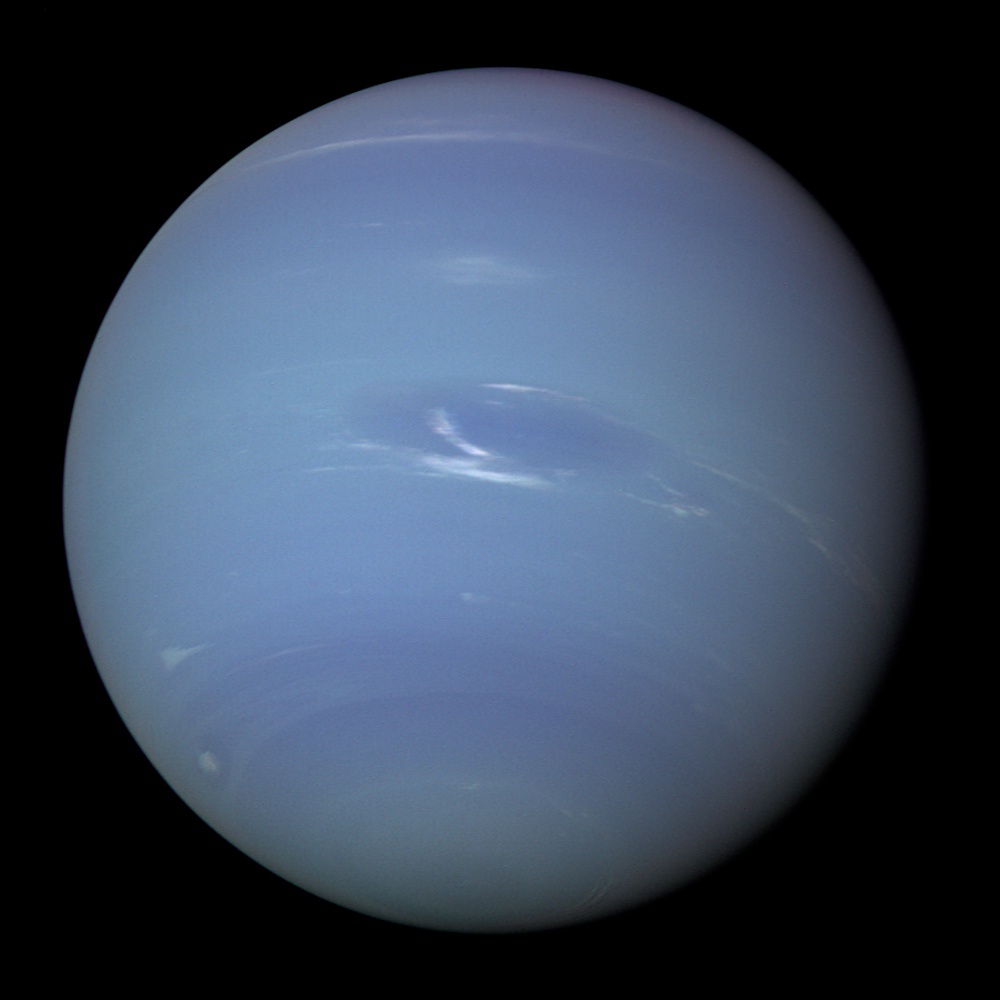
\includegraphics[width=0.65\textwidth]{figures/Neptune_-_Voyager_2_(29347980845)_flatten_crop.jpg} 
        \end{center}

        $\uparrow$ within $1^\circ$ of predicted location
        \end{column}
    \end{columns}
\footnotetext[1]{J.P. Nichol, ``The planet Neptune: an exposition and history''
1849}
\end{frame}
}


